% Generated by thesis/ch7/exp2/networks.py -- do not edit by hand.
\begin{sidewaysfigure}
  \centering
  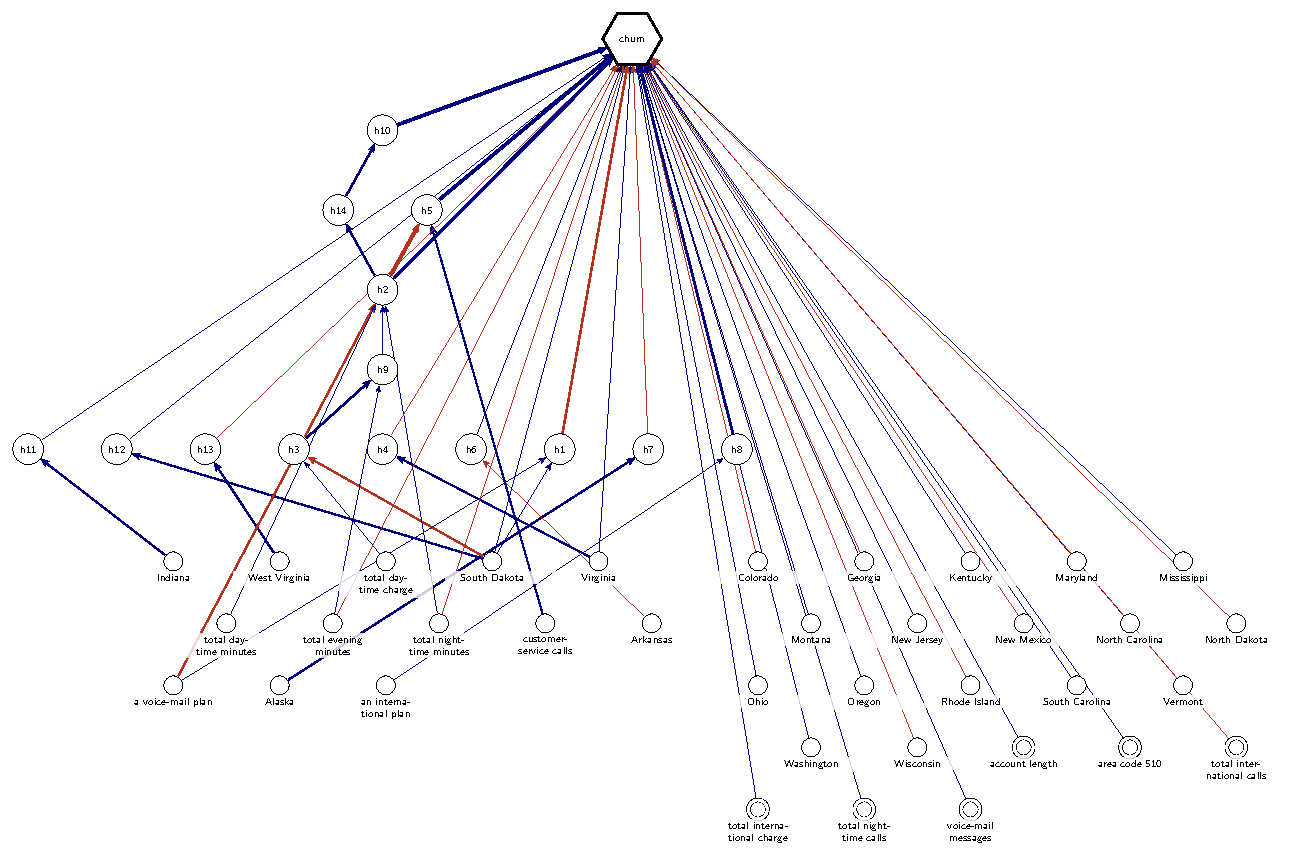
\includegraphics[width=\textheight,height=0.78\textwidth,keepaspectratio]{figures/exp2/networks/churn100-s7-raw}
  \caption{Churn, seed 7 (churn100-s7): the network as trained, before any explanation, in full. Inputs at the bottom (every input column its own node), hidden units by depth, the output at the top; 36 of 71 input columns are connected, with 14 hidden units and 59 enabled connections. Blue: positive weight (raises the score); red: negative weight (lowers it); thicker: larger weight. Orange outline and up arrow: raises the final prediction; teal and down arrow: lowers it; grey and double arrow: depends. Not used (no connection; 35 columns): Alabama, Hawaii, Iowa, Idaho, Illinois, Kansas, Louisiana, Massachusetts, Maine, Michigan, Minnesota, Missouri, Nebraska, Arizona, New Hampshire, Nevada, New York, Oklahoma, Pennsylvania, California, Tennessee, Texas, Utah, Wyoming, Connecticut, Washington DC, Delaware, Florida, area code 408, area code 415, total daytime calls, total evening calls, total evening charge, total night-time charge and total international minutes.}
  \label{fig:exp2-net-churn100-s7-raw}
\end{sidewaysfigure}
